\documentclass{standalone}
\usepackage{tikz}
\usepackage{ctex,siunitx}
\setCJKmainfont{Noto Serif CJK SC}
\usepackage{tkz-euclide}
\usepackage{amsmath}
\usetikzlibrary{patterns, calc}
\usetikzlibrary {decorations.pathmorphing, decorations.pathreplacing, decorations.shapes,}

\begin{document}
\small
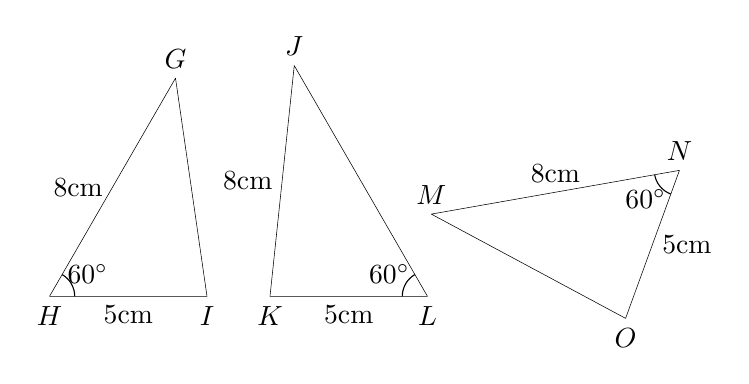
\begin{tikzpicture}[>=stealth,scale=0.8]
  \tkzSetUpPoint[fill=black]
  % \useasboundingbox(-1,-0.75)rectangle(3.7,1.4);
  \begin{scope}
  \tkzDefPoints{0/0/H, 2.5/0/I}
  \tkzDefPoint(60:4){G}
  \tkzDrawPolygon(H,I,G)
  \tkzLabelPoints[below](H,I)
  \tkzLabelPoints[above](G)
  \tkzLabelSegment[below](H,I){5cm}
  \tkzLabelSegment[left](H,G){8cm}
  \tkzMarkAngles[size=.4, mark=none](I,H,G)
  \tkzLabelAngle[pos=.7](I,H,G){$60^{\circ}$}
  \end{scope}
  \begin{scope}[xshift=6cm]
    \tkzDefPoints{0/0/L, -2.5/0/K}
  \tkzDefPoint(120:4.23){J}
  \tkzDrawPolygon(J,K,L)
  \tkzLabelPoints[below](K,L)
  \tkzLabelPoints[above](J)
  \tkzLabelSegment[below](K,L){5cm}
  \tkzLabelSegment[left](K,J){8cm}
  \tkzMarkAngles[size=.4, mark=none](J,L,K)
  \tkzLabelAngle[pos=.7](J,L,K){$60^{\circ}$}
  \end{scope}
  \begin{scope}[xshift=10cm, yshift=2cm, rotate=70]
    \tkzDefPoints{0/0/N, -2.5/0/O}
  \tkzDefPoint(120:4){M}
  \tkzDrawPolygon(M,N,O)
  \tkzLabelPoints[below](O)
  \tkzLabelPoints[above](M,N)
  \tkzLabelSegment[right](N,O){5cm}
  \tkzLabelSegment[above](M,N){8cm}
  \tkzMarkAngles[size=.4, mark=none](M,N,O)
  \tkzLabelAngle[pos=.7](M,N,O){$60^{\circ}$}
  \end{scope}
\end{tikzpicture}
\end{document}